% Chapter Template

\chapter{Modelo solo con RNN} % Main chapter title

\label{RNN} % Change X to a consecutive number; for referencing this chapter elsewhere, use \ref{ChapterX}

%----------------------------------------------------------------------------------------
%   SECTION 1
%----------------------------------------------------------------------------------------

\section{Primeros pasos}

Para estas pruebas, se utilizo en todo momento una red neural recurrente, proporcionada por el paquete NNET, para el lenguaje R.

Se comenzo realizando un pre procesado de los textos, como se había hablado en un inicio, en el cual se sacaron stopwords, se hizo un proceso de stemming y se dejo todo en un formato de texto plano.

Las primer idea, fue entrenar la red neuronal con una DTM TF, sin embargo, esto se vio rapidamente inviable.

La DTM completa poseía cerca de 10000 terminos, que no era un problema almacenarlos mientras pudieramos usar un formato de matriz hecho para matrices dispersas, sin embargo, para entrenar la red, se necesitaba una matriz en su formato tradicional.

El primer cambio realizado fue el mas trivial, quitar terminos cuya ocurrencia sea muy baja. Asi, se sacaron los terminos que aparecían con una frecuencia menor a 1 cada 100 documentos  y nos quedamos con aproximadamente 667 terminos.

Aún con esta cantidad, se tuvieron problemas de memoria, y la primer red neuronal fue entrenada con la mitad del set original, y utilizando un 80\% de los datos como train, y el resto como set.

El resultado fue cerca de un 14\% de precisión, la red neuronal no predecía.

\section{Primeras correcciones}

El error fue bastante evidente luego, nunca habíamos normalizado los datos. Decidimos entonces usar la normalización mas intuitiva. Aplicamos a todas las columnas la siguiente función:

\begin{equation}
z = \frac{x_{i}-min(x)}{max(x)-min(x)}
\end{equation}

Los resultados fueron igual de malos.

Entonces probamos otra una normalización gausseana, muchas veces llamada estandarización:

\begin{equation}
z = \frac{x_{i}-\mu(x)}{\sigma(x)}
\end{equation}

Y los resultados por primera vez fueron razonables. Redondeando los datos en el test se tuvo cerca de un 52\% de aciertos.

\section{Preparando para kaggle}

Para poder subir a Kaggle, necesitamos que nuestra red pueda predecir el test que tenemos. Sin embargo, se debe realizar la misma transformación a los datos que se le realizo al train. Para esto podíamos guardar los terminos y los datos de la media y el desvio estandar de cada de matriz, luego en el test quedarnos con esos terminos, y aplicar esa normalización. Siendo que solo nos interesa predecir un test, se decidio aprovechar para hacer todo esto, con el test y el train combinado.

Habiendo terminado eso, se subio la primer entrega a kaggle con un 1.15939 de error cuadrático medio.

\section{SVD}

Entrenar una red neuronal con una neurona, de la forma que veníamos haciendo era muy lento, y ocupaba mucho espacio en memoria. Por lo cual se decidio armar una SVD y quedarnos con los autovectores mas importante de la matriz u.

El primer inconveniente con esta idea, es que calcular la SVD, para la matriz DTM, excede nuestro poder computacional. Aún tirando terminos que se usan poco al principio. Si bien los métodos convenciales permiten cálcular menos vectores de U y de V, cálculan todos los autovalores. Y ahi se vuelve imposible 

Se recurrio entonces a otro algoritmo conocido como IRLBA, augmented implicitly restarted Lanczos bidiagonalization algorithm. Este nos permite cálcular nuestra SVD con la cantidad de autovectores y autovalores que necesitemos. Es extremedamente rápido para buscar los autovalroes mas grandes y sus autovectores asociados. Aunque es mas lento si se quiere computar toda la SVD, pero como eso nos era imposible, trabajamos con este método.

También posee la ventaja de poder reanudarse. Utilizando el resultado de la ultima iteración, se puede seguir calculando mas autovalores y autovectores de la SVD, por lo cual no se pierde el trabajo computado.

Cálculamos 170 autovectores y autovalores, con una noche completa de cálculo. Lo primero que hicimos fue ver como era la distribución de la energía, para ver cuanta información perderíamos al estimar con la SVD. Este fue el resultado:

\begin{figure}[h]
{
    \centering
    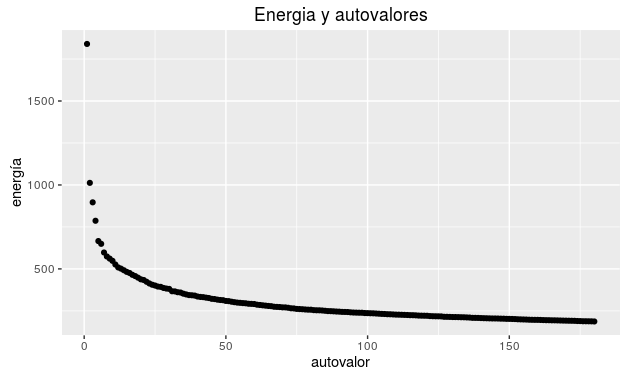
\includegraphics[width=1\linewidth]{Figures/svd.png}
}
Si lo ponemos en escala logaritmica\par\bigskip
{
    \centering
    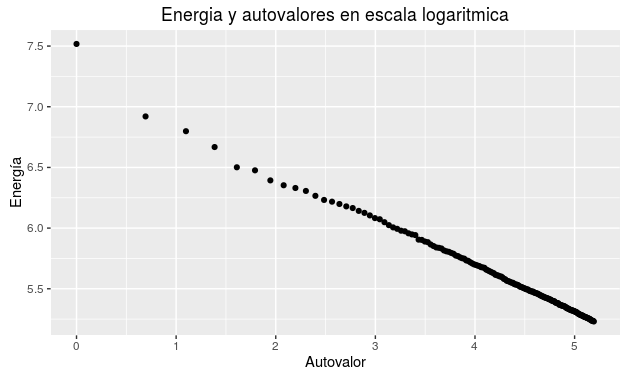
\includegraphics[width=1\linewidth]{Figures/svdLog.png}
}
\end{figure}

Lamentablemente, es una ley de potencias. La cola alargada que vemos, nos provoca que la energía comience a bajar muy de a poco. Y teniendo en cuenta que hay muchisimos terminos, el peso no es despreciable.

Aún así, siendo que de todas formas no podíamos utilizar todos los datos que teníamos, decidimos utilizar 50 columnas de la matriz u de la SVD para estimar los datos, y ver que sucede.

La velocidad a la que se entrena una red neuronal, y en consecuencia la cantidad de neuronas que podíamos utilizar, aumento considerablemente. Los resultados fueron un poco peores. 
Con una neurona y una capa, tal como fue el primero, se obtuvo en kaggle 1.32583 de RMSE. Recordamos que el original había sido 1.13817.

Sin embargo, aprovechando los nuevos tiempos de entrenamiento, se probo que pasaba si variabamos hiper parametros.

 
\section{Ajustando hiper parametrós}

Una primer prueba, solo por curiosidad, fue ver si había alguna diferencia cambiando de TF a IDF.

La red neuronal se entreno ligeramente mas rápido con IDF, y el resultado teniendo en cuenta la precisión fue:


TF - Precision en el Train: 55.3775 \%  
TF - Precision en el Test: 54.78959 \%

TF-IDF - Precision en el Train: 55.37\%  
TF-IDF  - Precision en el Test: 54.72912 \%

El cambio fue minimo. Se continuo usando TF que fue ligeramente superior.

Pasadas nuestras pequeñas pruebas, se planteo que había que automatizar la forma de ajustar hiper parametros. Y realizar una comparación mejor, que redondear los resultados.

Para esto utilizamos la librería Caret, y con ella, continuamos utilizando el mismo modelo. Ahora entrenamos con un two fold cross validation, y comparando con el error cuadratico medio. Trabajamos con una capa, y variamos la cantidad de neuronas y el decay. Para generar redes mas rápido, utilizamos una muestra del set. Al final entrenaremos con todo el set.

Elegimos two fold cross validation, porque si bien aumentamos la velocidad a la que calculamos una red neuronal, sigue sin ser despreciable el tiempo utilizado, mas cuando ahora la empezamos a complejizar. Por otro lado, configuramos el sistema para que compute distintas redes en diferentes nucleos y acelerar el proceso. También redujimos a un 20\% el set de entrenamiento, para poder computar más rápidamente las redes.

Este fue el primer resultado:

\begin{center}
    \begin{tabular}{| l | l | l | l |}
    \hline
    decay & size & RMSE & Rsquared \\ \hline
    0.000 & 1 & 1.164061 & 0.2123402 \\ 
    0.000 & 2 & 1.144628 & 0.2383667  \\
    0.000 & 10 & 1.145871 & 0.2401054  \\
    0.001 & 1 & 1.153106 & 0.2270361  \\
    0.001 & 2 & 1.155142 & 0.2251961  \\
    0.001 & 10 & 1.131491 & 0.2577052  \\
    0.010 & 1 & 1.152959 & 0.2272637  \\
    0.010 & 2 & 1.135215 & 0.2507921  \\
    0.010 & 10 & 1.131509 & 0.2572446  \\
    \hline
    \end{tabular}
\end{center}

Vemos que a medida que cuando aumenta la cantidad de neuronas el resultado en general mejora. Por otro lado, tener un poco de decay ayuda. Si bien el mejor resultado lo obtuvimos con un decay de 0.001, es en el caso de un decay de 0.01 donde siempre mejora el resultado, para todo tamaño de red. Y los valores son similares.

Agregamos entonces dos pruebas mas, con mas neuronas, y observamos que empeoro.

\begin{center}
    \begin{tabular}{| l | l | l | l |}
    \hline
    decay & size & RMSE & Rsquared \\ \hline
    0.01 & 20 & 1.136187 & 0.2557508 \\
    0.01 & 50 & 1.171565 & 0.2322588 \\
    \hline
    \end{tabular}
\end{center}

Entrenando conla muestra el resultado en kaggle fue de un RMSE de 1.26806. Y al entrenar con todo el train disponible llegamos a 1.20078. Un resultado que se empieza a acercar al primero.

